% !TEX program = pdflatex
% =====================================================================
%  Explicit finite-order lower bounds for high-order robust composite
%  Z rotations.
%  APS/REVTeX 4.2 manuscript, single-column submission format.
%  Build:  pdflatex main ; bibtex main ; pdflatex main ; pdflatex main
% =====================================================================
\documentclass[%
  aps,
  pra,
  preprint,
  superscriptaddress,
  amsmath,amssymb,
  nofootinbib,
  floatfix,
]{revtex4-2}

\usepackage[T1]{fontenc}
\usepackage[utf8]{inputenc}
\usepackage{lmodern}
\usepackage{graphicx}
\usepackage{bm}
\usepackage{booktabs}
\usepackage{enumitem}
\usepackage{microtype}
\usepackage{amsthm}
\usepackage[hidelinks,breaklinks]{hyperref}

\pdfstringdefDisableCommands{%
  \def\lambda{lambda}\def\tau{tau}\def\phi{phi}\def\alpha{alpha}%
  \def\eps{epsilon}\def\C{C}\def\R{R}\def\lean#1{#1}\def\mathrm#1{#1}%
}

% ---------------------------------------------------------------- macros
\newtheorem{theorem}{Theorem}
\newtheorem{lemma}[theorem]{Lemma}
\newtheorem{proposition}[theorem]{Proposition}
\newtheorem{corollary}[theorem]{Corollary}
\theoremstyle{definition}
\newtheorem{definition}[theorem]{Definition}
\theoremstyle{remark}
\newtheorem{remark}[theorem]{Remark}

\newcommand{\Tr}{\operatorname{Tr}}
\newcommand{\Ree}{\operatorname{Re}}
\newcommand{\norm}[1]{\left\lVert #1\right\rVert}
\newcommand{\Lone}[1]{\left\lVert #1\right\rVert_{L^1}}
\newcommand{\C}{\mathbb C}
\newcommand{\R}{\mathbb R}
\newcommand{\eps}{\varepsilon}
\newcommand{\tauvar}{\tau}
\newcommand{\cstar}{c_*}
\newcommand{\supp}{\operatorname{supp}}
\newcommand{\e}{\mathrm e}
% Names of Lean declarations and of files of the formal development.
\DeclareRobustCommand{\lean}[1]{\path{#1}}
% Ragged-right table cell (\\ stays the row separator, as \arraybackslash would do).
\newcommand{\raggedcell}{\raggedright\let\\\tabularnewline}

\allowdisplaybreaks

\begin{document}

\title{Explicit finite-order lower bounds for\\
high-order robust composite $Z$ rotations}

\author{Dytchem}
\affiliation{Independent researcher}
\thanks{Corresponding author: contact through the public project page
\url{https://github.com/Dytchem/robust-z-lower-bound-lean}.}
\date{October 2026}

\begin{abstract}
We study the unavoidable cost of a high-order robust single-qubit $Z$ rotation in a
minimal model: the $Z$ evolution is imperfect, its angle carrying a common unknown
multiplicative error, while exact, instantaneous and free $X$ rotations are available in
unlimited number and at arbitrary positions. The resource is the total nominal $Z$ angle
$T$. We prove explicit lower bounds on $T$ that hold at every order $N$ of error
cancellation, with all constants written out; they form a ladder of four rungs with
asymptotic coefficients $2/\e$, $4/\e$, $2\pi/\e$ and $4$. The first two rungs follow from a
single Taylor step, applied first to the propagator and then to the scalar endpoint
separation whose vanishing order the unitary structure doubles. The third applies Jensen's
formula to the carrier, an entire function of exponential type whose bandwidth is half the
cost. The fourth replaces the vanishing derivatives by vanishing moments and approximates
the carrier's phase on its whole frequency band. That last rung is an exact, checkable
criterion: whenever an explicit closed-form quantity in the bandwidth falls below
$\sin^2(\phi/4)$, every order-$N$ sequence satisfies $T>2\tau$. It certifies, with
machine-checked arithmetic and no approximation-theory input, the bounds
$T\ge2,2,4,8,10,14,16,18,22,24,28$ at $\phi=\pi$ for $N=2,\dots,12$, and its closed form
gives the asymptotic coefficient $4$. We also delimit the method: whether any argument
that uses only the bandwidth and the flatness order can pass $4$ is equivalent to an explicit
uncertainty-principle-type statement, the remaining gap is the interval $[4,2\pi]$, and
incoherent errors of a real device place the useful order near $N=2$--$4$. All bounds beyond the first rung are formalized in Lean~4 with Mathlib, as per-sequence
statements.
\end{abstract}

\keywords{robust quantum control; composite pulses; systematic error; linear lower bound;
Fourier approximation; formal verification; Lean}

\maketitle

\section{Introduction}
\label{sec:intro}

Composite-pulse methods suppress systematic control errors by replacing a single imperfect
operation with a structured sequence whose error terms cancel order by order. Arbitrarily
high-order cancellation was established in early work on composite pulses, and the optimal
asymptotic scaling of the number of primitive pulses was later characterized for important
pulse-length-error models~\cite{Brown2004,Merrill2014,Low2014}. A separate line of work has
addressed lower bounds on the physical operation time of robust composite gates, including
geometric bounds for first-order pulse-length-error robustness~\cite{Kukita2023} and time
lower bounds for first-order robustness under bounded control amplitude~\cite{Zeng2025,Kosut2025}.
Order-$N$ cancellation is the vanishing of the first $N$ error moments, the condition that
also underlies optimized dynamical decoupling and the filter-function description of
open-loop control~\cite{Kabytayev2014,Uhrig2007,PazSilva2014}, where rigorous design bounds
of a different type are available~\cite{UhrigLidar2010,Khodjasteh2011,NgLidarPreskill2011}.
Section~\ref{sec:related} compares these formulations with the one used here.

The resource model considered here is deliberately different. Suppose that one available
interaction generates a $Z$ rotation but its strength is not known exactly, and that a second
control can rotate the system about an orthogonal $X$ axis with sufficiently high precision
that, in the idealized limit, its duration may be regarded as negligible. The natural
question is then not how many control pulses are needed, but how much of the imperfect
interaction must unavoidably be accumulated in order to cancel the common systematic error to
a specified order. The distinction matters: a lower bound on the number of primitive
rotations does not immediately give a lower bound on a time resource when some rotations are
assigned zero cost.

The setting also occurs naturally in Rydberg-atom control. In a recent QSP-based
proposal~\cite{Ye2026}, the interaction between two Rydberg atoms is treated as an unknown but
deterministic phase input, while fast Rydberg transitions are used as interleaved controls,
and systematic variation of the interaction strength is suppressed by composite control.
Systematic control deviations are, independently of that proposal, among the dominant error
sources of neutral-atom two-qubit gates~\cite{Evered2023,Mohan2023}. The present work isolates
the single-qubit mathematical core of this setting: what is the unavoidable amount of an
uncertain $Z$ evolution if exact transverse rotations are free?

The results proved here are explicit, finite-order statements: lower bounds on $T$ that hold
at every prescribed order $N$, with all constants written out. They form a ladder of four
rungs, in the order $2/\e\to4/\e\to2\pi/\e\to4$, each using strictly more of the structure of
the problem than the previous one. Differentiating the propagator itself and taking one
Taylor--Lagrange step at the endpoint gives
$T\ge2\,[\,2\,(N+1)!\,\sin(\phi/4)\,]^{1/(N+1)}$, a coefficient $2/\e$ in $N$; this rung uses
nothing but the product rule, and it is kept to show how little is needed for linear growth.
Doubling the flatness through a scalar carrier turns the same step into
$T\ge2\,[\,2\,q!\,\sin^{2}(\phi/4)\,]^{1/q}$ with $q=2N+2$, a coefficient
$4/\e\approx1.4715$ (Theorem~\ref{thm:elementary}). The carrier extends to an entire function
of exponential type $T/2$, so Jensen's formula converts the same $q$-fold zero at the nominal
point into $T\ge\pi q/[\e\,(2/s)^{1/q}]$ with $s=2\sin^{2}(\phi/4)$, a coefficient
$2\pi/\e\approx2.3115$ with no threshold and no approximation theory
(Theorem~\ref{thm:jensen}). Finally, the vanishing derivatives become $q$ vanishing moments,
into which any polynomial of degree $q-1$ may be inserted; approximating $\e^{-\mathrm{i}\mu}$
on the whole band and smoothing with a compactly supported Fourier multiplier makes the
endpoint value exponentially small whenever an explicit closed-form criterion in the bandwidth
is met, which contradicts the order-one separation of the endpoint and yields a checkable
certificate $T>2\tau$ at every order (Theorem~\ref{thm:newrung}), together with a
Lean-certified finite-$N$ table and a closed form whose coefficient approaches $4$. The four
bounds combine into a single bound valid at every order (Corollary~\ref{cor:allN}), from which
$\liminf_{N\to\infty}T_{\min}(N,\phi)/N\ge4$ follows.

The control model, admissibility, the achievable costs, the carrier, and the three rungs beyond
the first are contained in public Lean~4 + Mathlib developments~\cite{LeanRepo}; the paper
follows those developments closely, and Sec.~\ref{sec:formal} lists what is machine-checked,
statement by statement.

The paper is organized as follows. Section~\ref{sec:related} reviews the relation to previous
work. Section~\ref{sec:model} states the model and all four bounds up front, with no proofs.
Sections~\ref{sec:elementary}--\ref{sec:newrung} prove the rungs in ladder order, one rung
family per section, with the shared carrier setup factored once into Sec.~\ref{sec:carrier} and
cited thereafter. Section~\ref{sec:numerics} reports numerical sequences as upper bounds only,
with no optimality claim. Section~\ref{sec:formal} tabulates the correspondence with the formal
development, and Section~\ref{sec:discussion} records what cannot improve the ladder, the open
ceiling dichotomy at $4$, and the orders that matter for a device. The appendices collect the
closed forms and the kernel estimate behind the exact criterion, and the conventions of the
numerical data.

\section{Relation to Previous Work}
\label{sec:related}

The earliest composite-pulse constructions showed that systematic pulse-length errors can be
cancelled to arbitrarily high order~\cite{Brown2004}, and Ref.~\cite{Merrill2014} reviews the
vocabulary of order-$N$ robustness and of cost accounting in that setting. Low, Yoder, and
Chuang subsequently proved that, in a standard primitive-pulse model, the number of primitive
rotations required for arbitrary accuracy has optimal linear scaling in the robustness order,
with constructions saturating that scaling~\cite{Low2014}. Their statement has the same shape
as Theorem~\ref{thm:newrung}---a linear lower bound in the robustness order together with a
construction that saturates it---but the resource there is the number of primitive rotations,
in a model where those rotations are themselves part of the costly control sequence. It
therefore says nothing about the minimum $Z$-evolution time in the free-$X$ model, which is the
resource bounded here.

The identification of order-$N$ error cancellation with the vanishing of the first $N$ moments
of the error is standard in dynamical decoupling and in the filter-function description of
open-loop control: it is the defining condition of Uhrig's optimized
sequences~\cite{Uhrig2007}, and it was put on a general footing by the transfer-function
analysis of Ref.~\cite{PazSilva2014}. The composite-pulse counterpart, a single-qubit sequence
analyzed order by order in its systematic pulse-length error, is treated
in Ref.~\cite{Kabytayev2014}. Section~\ref{sec:newrung} uses the same identity, but the carrier
there is a function of a $Z$-evolution budget rather than of a pulse train, and the constant $4$
comes from the fact that this carrier is band-limited.

Kukita, Kiya, and Kondo derived a lower bound on the operation time of first-order
pulse-length-error robust composite gates from a geometric argument~\cite{Kukita2023}. In their
resource model the rotations that change the control axis cost time; here they are instantaneous
and free, so a geometric bound on the full control path is not a bound on $T$.

Two recent works bound noise-robust control from the side of the control amplitude. Zeng and
Deng prove a universal average-case time lower bound for first-order robustness against a
single quasistatic coherent error under bounded control amplitude, together with a construction
that is robust in time $4T$ plus a constant~\cite{Zeng2025}; that overhead is fixed and
$N$-independent, whereas the coefficient studied here is linear in the robustness order. Kosut,
Lidar, and Rabitz prove a universal lower bound on the fidelity of any robustly controlled gate
as a function of the gate duration times an aggregate uncertainty~\cite{Kosut2025}. Both
concern first-order or order-independent robustness, and neither is sharp in the way the rungs
are for the model of Sec.~\ref{sec:model}: the present proof uses the analytic dependence on a
common scale parameter $\lambda$ and holds for arbitrary order $N$.

Machine-checked quantum information is by now a developed subject---quantum programs and
compilers in Coq and Isabelle/HOL~\cite{Bordg2021}, and quantum information theory in
Lean~\cite{Meiburg2025}---but we are not aware of a formalized lower bound in quantum control.
The developments behind Theorems~\ref{thm:elementary}, \ref{thm:jensen}
and~\ref{thm:newrung} attempt one, for a model small enough that the whole proof, analytic
estimates included, is checked by the kernel.

The connection to the supplied Rydberg QSP manuscript~\cite{Ye2026}---unpublished at the time
of writing---is complementary. That work treats an unknown interaction phase as the input to a
QSP-style composite protocol and uses fast control pulses to suppress systematic interaction
variation. The present result identifies a resource limitation in the idealized single-axis
core of that philosophy: even with perfect free transverse controls, high-order cancellation
cannot be made sublinear in the amount of uncertain evolution.

\section{Control model and main results}
\label{sec:model}

\subsection{Elementary rotations and composite sequences}

Let
\begin{equation}
X(\alpha):=\exp\!\left(-\mathrm{i}\frac{\alpha}{2}\sigma_x\right),
\qquad
Z(\theta):=\exp\!\left(-\mathrm{i}\frac{\theta}{2}\sigma_z\right),
\label{eq:rotations}
\end{equation}
where $\sigma_x$ and $\sigma_z$ are the Pauli matrices. Throughout, $\lVert\cdot\rVert$ is the
operator norm on matrices (the largest singular value), which equals one on unitary matrices, and
all numerics reported in Sec.~\ref{sec:numerics} use the same norm. The $X$ rotations are assumed exact,
instantaneous, and free. The $Z$ evolution is the only costly operation, and in the presence of a
fixed unknown fractional error $\eps$ its actual propagator is
\begin{equation}
Z^{\eps}(\theta)
=\exp\!\left[-\mathrm{i}\frac{(1+\eps)\theta}{2}\sigma_z\right].
\label{eq:imperfectZ}
\end{equation}

For $L\ge0$, choose real angles $\alpha_j$ and nonnegative $Z$ angles $\theta_j$. Following the
recursive order used in the Lean development, define
\begin{equation}
U_\lambda
= X(\alpha_1)Z(\lambda\theta_1)
  X(\alpha_2)Z(\lambda\theta_2)\cdots
  X(\alpha_L)Z(\lambda\theta_L),
\label{eq:sequence}
\end{equation}
with $U_\lambda=I$ for $L=0$. Relabeling the indices gives the equivalent convention in which
$X(\alpha_L)Z(\lambda\theta_L)\cdots X(\alpha_1)Z(\lambda\theta_1)$ is written from left to right.
Nothing in the proof depends on this notational choice.

The parameter $\lambda$ is an interpolation variable: the physical propagator at error $\eps$ is
$U_{1+\eps}$. The target is
\begin{equation}
U_1=Z(\phi),\qquad 0<\phi\le\pi.
\label{eq:target}
\end{equation}
The cost is the total nominal $Z$ angle,
\begin{equation}
T:=\sum_{j=1}^L\theta_j.
\label{eq:cost}
\end{equation}
The normalization is chosen so that the nominal $Z$ rotation rate is one; restoring a physical
rate $\omega$ simply replaces $T$ by $T/\omega$ in the time interpretation.

\begin{definition}[Order-$N$ robustness]
\label{def:admissible}
A sequence is \emph{order-$N$ admissible for $\phi$} if
$\theta_j\ge0$, $U_1=Z(\phi)$, and
\begin{equation}
\left.\frac{\mathrm{d}^k U_\lambda}{\mathrm{d}\lambda^k}\right|_{\lambda=1}=0,
\qquad k=1,\ldots,N.
\label{eq:robustness}
\end{equation}
This is exactly matrix-valued flatness at the nominal error point.
\end{definition}

Let $\mathrm{costs}(N,\phi)$ denote the set of costs of all admissible sequences and define
mathematically
\begin{equation}
T_{\min}(N,\phi):=\inf\mathrm{costs}(N,\phi),
\qquad
\cstar(\phi):=\liminf_{N\to\infty}\frac{T_{\min}(N,\phi)}{N}.
\label{eq:tmin}
\end{equation}

\begin{theorem}[First rung, direct Taylor bound, paper-level]
\label{thm:direct}
For every $0<\phi\le\pi$ and every order-$N$ admissible sequence,
\begin{equation}
\displaystyle
T\ge
2\left[2(N+1)!\sin\left(\frac\phi4\right)\right]^{1/(N+1)}.
\label{eq:2e-finite}
\end{equation}
Using Stirling's formula,
$(N+1)!^{1/(N+1)}=(N+1)\mathrm{e}^{-1}(1+o(1))$, and the fixed factor
$[2\sin(\phi/4)]^{1/(N+1)}$ tends to one. Hence
\begin{equation}
\cstar(\phi)\ge\frac{2}{\mathrm{e}}.
\label{eq:2e}
\end{equation}
This rung is paper-level; it is pointwise weaker than Theorem~\ref{thm:elementary} at every
order and is omitted from the maximum in Corollary~\ref{cor:allN}.
\end{theorem}

\begin{theorem}[Elementary bound, valid at every order]
\label{thm:elementary}
For every $0<\phi\le\pi$ and every order-$N$ admissible sequence,
\begin{equation}
\displaystyle
T\;\ge\;2\,\Bigl[\,2\,(2N+2)!\,\sin^{2}\!\Bigl(\frac{\phi}{4}\Bigr)\Bigr]^{1/(2N+2)} .
\label{eq:thm-elementary}
\end{equation}
In particular, at $\phi=\pi$, $T\ge 2\,[(2N+2)!]^{1/(2N+2)}$, which exceeds $4(N+1)/\mathrm{e}$ at every
order; the limiting coefficient of $N$ is $4/\mathrm{e}\approx1.4715$. This bound holds at every order
with no threshold, no approximation theory, and no transcendental input beyond the
factorial and a $q$-th root. It is machine-checked as \lean{elementary_bound} (see
Sec.~\ref{sec:formal}).
\end{theorem}

\begin{theorem}[Jensen bound, valid at every order]
\label{thm:jensen}
Write $q=2N+2$ and $s=2\sin^2(\phi/4)$. For every $0<\phi\le\pi$ and every order-$N$
admissible sequence,
\begin{equation}
\displaystyle
T\;\ge\;\frac{\pi\,q}{\mathrm{e}\,(2/s)^{1/q}} .
\label{eq:thm-jensen}
\end{equation}
In particular, at $\phi=\pi$, $T\ge\pi q/(\mathrm{e}\,2^{1/q})$; the limiting coefficient of $N$ is
$2\pi/\mathrm{e}\approx2.3115$. The bound is explicit at every order, with deficit only
$(2/s)^{1/q}-1$ vanishing as $q\to\infty$. It is machine-checked as \lean{jensen_rung_final}
(and \lean{jensen_rung_pi_final} at $\phi=\pi$); the per-$N$ bound divided by $N$ tends to
$2\pi/\mathrm{e}$ (Lean \lean{jensen_ratio_tendsto}).
\end{theorem}

\begin{theorem}[Exact-criterion rung, valid at every order]
\label{thm:newrung}
Let $N\ge1$, $q=2N+2$, $0<\phi\le\pi$, and $1\le\tauvar<q$. With the explicit closed-form
quantities $\mathrm{nrCcal}(\tauvar,q)$ and $\mathrm{nrE2star}(\tauvar,q)$ of
Appendix~\ref{app:technical}, if
\begin{equation}
\displaystyle
\mathrm{nrCcal}(\tauvar,q)\,q^2\,\mathrm{nrE2star}(\tauvar,q)
\;<\;\sin^2\!\Bigl(\frac{\phi}{4}\Bigr),
\label{eq:thm-newrung}
\end{equation}
then every order-$N$ admissible sequence for the target $\phi$ satisfies
\begin{equation}
T\;>\;2\tauvar,
\qquad\text{hence for all admissible sequences at every }N.
\label{eq:newrung-conclusion}
\end{equation}
The statement is machine-checked as \lean{new_rung_final}: the hypothesis is the strict
inequality $\tauvar<q$ with $1\le\tauvar$, and the conclusion is the strict bound
$2\tauvar<\mathrm{cost}\,\theta$. No threshold profile and no $a$-parameter enter: any
$\tauvar$ passing the check certifies $T>2\tauvar$.
\end{theorem}

\begin{corollary}[A single bound at every order]
\label{cor:allN}
For every $N\ge1$ and every $0<\phi\le\pi$, every order-$N$ admissible sequence satisfies
\begin{equation}
T\;\ge\;\max\Bigl\{\;2\,\bigl[\,2\,q!\,\sin^2(\phi/4)\bigr]^{1/q},\;
\pi q/(\mathrm{e}(2/s)^{1/q}),\;
2\,\tauvar^\ast\Bigr\},
\label{eq:allN}
\end{equation}
where $s=2\sin^2(\phi/4)$ and
$\tauvar^\ast=\sup\{\tauvar\in[1,q):\mathrm{nrCcal}(\tauvar,q)\,q^2\,
\mathrm{nrE2star}(\tauvar,q)<\sin^2(\phi/4)\}$.
Consequently $\cstar(\phi)\ge4$; the Lean developments state the three per-sequence bounds
in~\eqref{eq:allN} (the paper-level $2/\mathrm{e}$ first rung of Theorem~\ref{thm:direct} is
pointwise weaker than Theorem~\ref{thm:elementary} and is omitted from the maximum),
and the passage to $\cstar$ is elementary analysis. All rungs used here cover
$0<\phi\le\pi$; only the certified finite-$N$ table below is stated at $\phi=\pi$.
\end{corollary}

Table~\ref{tab:twolayers} compares the four rungs at sample orders. The Jensen rung is the
strongest of them at every tabulated order $N\le12$, and the exact-criterion rung takes over
asymptotically, where its coefficient $4$ exceeds $2\pi/\mathrm{e}$; the ratio of the two rows
tends to $\pi/2$. The first three rows evaluate the closed
forms~\eqref{eq:2e-finite}--\eqref{eq:thm-jensen}, whereas the last row consists of integers
proved inside Lean (Sec.~\ref{sec:newrung}), not of evaluations.

\begin{table}[t]
\centering
\small
\caption{The four rungs of the ladder---Theorems~\ref{thm:direct}, \ref{thm:elementary},
\ref{thm:jensen} and~\ref{thm:newrung}---at $\phi=\pi$ and sample orders $N$, with $q=2N+2$.
Rows: direct, $2\,[(N+1)!\,\sqrt2\,]^{1/(N+1)}$ (paper-level); elementary, $2\,(q!)^{1/q}$
(\lean{elementary_bound_pi}); Jensen, $\pi q/(\mathrm{e}\,2^{1/q})$
(\lean{jensen_rung_pi_final}); last row, the integers $2\tauvar$ certified in Lean
(\lean{cert_N2}--\lean{cert_N4}, \lean{cert_N5_tight}--\lean{cert_N12_tight}). Bold marks the
strongest proved lower bound at each order.}
\label{tab:twolayers}
\begin{tabular}{lrrrrrrrr}
\toprule
$N$ & $2$ & $3$ & $4$ & $5$ & $6$ & $8$ & $10$ & $12$\\
\midrule
direct (paper-level) & $4.08$ & $4.83$ & $5.58$ & $6.34$ & $7.10$ & $8.62$ & $10.13$ & $11.64$\\
elementary & $5.99$ & $7.53$ & $9.06$ & $10.58$ & $12.09$ & $15.11$ & $18.11$ & $21.10$\\
Jensen & $\mathbf{6.18}$ & $\mathbf{8.48}$ & $\mathbf{10.78}$ & $\mathbf{13.09}$ & $\mathbf{15.40}$ & $\mathbf{20.02}$ & $\mathbf{24.64}$ & $\mathbf{29.26}$\\
exact-criterion cert & $2$ & $2$ & $4$ & $8$ & $10$ & $16$ & $22$ & $28$\\
\bottomrule
\end{tabular}
\end{table}

\section{The carrier and the first two rungs}
\label{sec:elementary}

This section establishes the two cheapest rungs of the ladder and, with them, the fact that
high-order robustification cannot be sublinear in the order. Both rungs need only one scalar
object, the carrier $h(\lambda)=1-\tfrac12\Ree\Tr(U_1^\dagger U_\lambda)$ of
Sec.~\ref{sec:carrier}: order-$N$ matrix flatness at the nominal point makes $h$ flat there to
order $q=2N+2$, while the derivatives of $h$ are bounded by powers of the bandwidth
$\tauvar=T/2$. One Taylor step at the endpoint $\lambda=0$, where the costly evolution is
switched off, then gives the paper-level bound
$T\ge2\,[\,2\,(N+1)!\,\sin(\phi/4)\,]^{1/(N+1)}$ (Sec.~\ref{sec:direct}) and, with the
doubled flatness order, the bound $T\ge2\,[\,2\,q!\,\sin^{2}(\phi/4)\,]^{1/q}$
(Sec.~\ref{sec:doubled}). Their asymptotic coefficients differ by exactly the factor by which
the flatness order doubles.

\subsection{Carrier setup (once)}
\label{sec:carrier}

Set
\begin{equation}
\tauvar:=\frac{T}{2},
\qquad q:=2N+2,
\label{eq:tauq}
\end{equation}
and introduce the carrier
\begin{equation}
h(\lambda):=
1-\frac12\Ree\Tr\!(U_1^\dagger U_\lambda).
\label{eq:h}
\end{equation}
Normalized in this way, $h$ carries everything the two rungs need: it measures the separation
of the endpoints, its vanishing order at the nominal point is twice the order of the matrix
flatness, and it is a finite exponential sum of bandwidth $\tauvar$.

\subsubsection{Finite exponential bandwidth}

Because
\[
Z(\lambda\theta)
=\mathrm{e}^{-\mathrm{i}\lambda\theta/2}\frac{I+\sigma_z}{2}
 +\mathrm{e}^{+\mathrm{i}\lambda\theta/2}\frac{I-\sigma_z}{2},
\]
expanding the product in~\eqref{eq:sequence} shows that every matrix element of $U_\lambda$ is a
finite sum of exponentials $\mathrm{e}^{\mathrm{i}\mu\lambda}$ with
\begin{equation}
\mu=\frac12\sum_{j=1}^L s_j\theta_j,
\qquad s_j\in\{-1,+1\}.
\end{equation}
Consequently,
\begin{equation}
h(\lambda)=\sum_m \gamma_m \mathrm{e}^{\mathrm{i}\mu_m\lambda},
\qquad |\mu_m|\le\tauvar.
\label{eq:expsum}
\end{equation}
Thus $T/2$ is the bandwidth of the carrier: no component of $h$ oscillates faster than
$\tauvar$.

\subsubsection{Bounds on the carrier}

The relative propagator $V_\lambda:=U_1^\dagger U_\lambda$ is unitary. Therefore
$|\Tr V_\lambda/2|\le1$, and hence
\begin{equation}
0\le h(\lambda)\le2.
\label{eq:h-bounds}
\end{equation}
At the nominal point $\lambda=1$, $V_1=I$. Write locally
\[
V_\lambda=a(\lambda)I+\mathrm{i}\bm b(\lambda)\cdot\bm\sigma,
\qquad a^2+|\bm b|^2=1,
\]
with $a(1)=1$ and $\bm b(1)=0$. Matrix flatness of $U_\lambda$ through order $N$ implies
flatness of $V_\lambda$ through order $N$, so $\bm b$ has a zero of order at least $N+1$ at
$\lambda=1$. Since
\[
h=1-a=\frac{1-a^2}{1+a}
=\frac{|\bm b|^2}{1+a},
\]
and the denominator does not vanish near $\lambda=1$, the vanishing order of $h$ is twice that
of $\bm b$, hence at least $2N+2$. This doubling is what the second rung exploits.

\begin{proposition}[Carrier flatness]
\label{prop:flatness}
For an order-$N$ admissible sequence,
\begin{equation}
h^{(k)}(1)=0,
\qquad k=0,1,\ldots,q-1,
\qquad q=2N+2.
\label{eq:hflat}
\end{equation}
In particular, the scalar flatness is a consequence of the matrix flatness and is not an additional
assumption.
\end{proposition}

\subsubsection{The endpoint at \texorpdfstring{$\lambda=0$}{lambda=0}}

At $\lambda=0$, all $Z$ factors become the identity, and therefore
\begin{equation}
U_0=X(A),
\qquad A:=\sum_{j=1}^L\alpha_j.
\label{eq:u0}
\end{equation}
The target endpoint is $U_1=Z(\phi)$. A direct $SU(2)$ calculation gives
\begin{equation}
\Tr\![Z(\phi)^\dagger X(A)]
=2\cos\frac\phi2\cos\frac A2.
\end{equation}
Hence
\begin{equation}
\displaystyle
h(0)=1-\cos\frac\phi2\cos\frac A2.
\label{eq:h0exact}
\end{equation}
For $0<\phi\le\pi$, $\cos(\phi/2)\ge0$, so
\begin{equation}
h(0)\ge1-\cos\frac\phi2
=2\sin^2\frac\phi4>0.
\label{eq:h0lower}
\end{equation}
The distinction matters: the sharper-looking identity $h(0)=1-\cos(\phi/2)$ is false in
general, because the free $X$ rotations leave the arbitrary factor $\cos(A/2)$.

There is also a useful geometric interpretation. For $U,V\in SU(2)$,
\begin{equation}
\norm{U-V}^2=2-\Tr(U^\dagger V),
\end{equation}
so, in the present case,
\begin{equation}
h(0)=\frac12\norm{U_1-U_0}^2.
\label{eq:h-distance}
\end{equation}
Thus the lower bound~\eqref{eq:h0lower} says that the target is uniformly separated from the
set of endpoint propagators obtainable by turning off the costly $Z$ evolution.

\subsection{Direct propagator estimate: \texorpdfstring{$2/\mathrm{e}$}{2/e}}
\label{sec:direct}

This is the first rung of the ladder. It is paper-level: one Taylor step
without doubling. Differentiating a single $Z$ factor gives
\[
\norm{\frac{\mathrm{d}^m}{\mathrm{d}\lambda^m}Z(\lambda\theta_j)}
=\left(\frac{\theta_j}{2}\right)^m.
\]
Applying the product rule to the whole sequence and using the unitarity of all undifferentiated
factors gives the multinomial estimate
\begin{equation}
\norm{U_\lambda^{(k)}}
\le
\sum_{k_1+\cdots+k_L=k}
\frac{k!}{k_1!\cdots k_L!}
\prod_j\left(\frac{\theta_j}{2}\right)^{k_j}
=\tauvar^k.
\label{eq:Ukbound}
\end{equation}
Taylor's theorem about $\lambda=1$, using the first $N$ vanishing derivatives, gives
\begin{equation}
\norm{U_0-U_1}
\le\frac{\tauvar^{N+1}}{(N+1)!}.
\label{eq:taylorU}
\end{equation}
On the other hand, $U_0=X(A)$ and $U_1=Z(\phi)$, and the exact endpoint geometry gives
\begin{equation}
\norm{X(A)-Z(\phi)}
\ge2\sin\frac\phi4.
\end{equation}
Together these prove Theorem~\ref{thm:direct}, stated in Sec.~\ref{sec:model}.

This already rules out sublinear robustification: arbitrarily high-order cancellation costs at
least $\Omega(N)$, and that conclusion needs nothing beyond the product rule and one Taylor
step. The bound is pointwise weaker than Theorem~\ref{thm:elementary} at every order, so it is
omitted from the maximum in Corollary~\ref{cor:allN}.

\subsection{Using the doubled flatness: \texorpdfstring{$4/\mathrm{e}$}{4/e}}
\label{sec:doubled}

The gain comes from the doubled flatness order. From~\eqref{eq:Ukbound} and
$|\Tr M|\le2\norm M$, one obtains
\begin{equation}
|h^{(k)}(\lambda)|\le\tauvar^k.
\label{eq:hkbound}
\end{equation}
By Proposition~\ref{prop:flatness}, the first $q-1$ derivatives of $h$ vanish at $1$, where
$q=2N+2$. Taylor's theorem therefore yields
\begin{equation}
|h(0)|\le\frac{\tauvar^q}{q!}.
\label{eq:taylorh}
\end{equation}
Combining with~\eqref{eq:h0lower} gives
\begin{equation}
\displaystyle
T\ge
2\left[2q!\sin^2\left(\frac\phi4\right)\right]^{1/q},
\qquad q=2N+2.
\label{eq:4e-finite}
\end{equation}
Since $(q!)^{1/q}\sim q/\mathrm{e}$, more precisely $(q!)^{1/q}=(q/\mathrm{e})(1+o(1))$,
\begin{equation}
\cstar(\phi)\ge\frac{4}{\mathrm{e}}\approx1.4715.
\label{eq:4e}
\end{equation}

The factor of two in the asymptotic coefficient comes entirely from the doubled flatness order
$q=2(N+1)$; no new physical assumption enters. The one piece of information still unused is that
$h$ is not merely flat and bounded but band-limited. Sec.~\ref{sec:jensen} converts the
bandwidth into a further factor $\pi/2$, giving the coefficient $2\pi/\mathrm{e}$, and
Sec.~\ref{sec:newrung} uses the whole band rather than one Taylor remainder point to reach a
coefficient approaching $4$.

\section{The Jensen rung}
\label{sec:jensen}

The carrier $h$ of~\eqref{eq:h} is a finite exponential sum, hence the restriction to
$\lambda\in\R$ of an entire function. Let $H$ be its canonical complexification. Only two
analytic facts about $H$ are needed: a growth bound in the imaginary direction, and Jensen's
formula on discs. Write $\tauvar=T/2$ and $s=2\sin^2(\phi/4)$, so that $h(0)\ge s>0$
by~\eqref{eq:h0lower}.

\subsection{Complex growth and zero counting}

Let $H$ be the canonical complexification of $h$. It is entire and satisfies the pointwise
growth bound
\begin{equation}
\|H(z)\|\;\le\;2\,\mathrm{e}^{\tauvar\,|\Im z|},
\qquad z\in\C,
\label{eq:jgrow}
\end{equation}
since each $X$ factor is unitary and each
$Z$ factor has norm $\mathrm{e}^{|y|\theta_j/2}$, so submultiplicativity gives the bound with no
dependence on the number of segments. Averaging $\log|H|$ over the circle $|z|=r$,
the indicator mean $\frac1{2\pi}\int_0^{2\pi}|\sin\theta|\,\mathrm{d}\theta=2/\pi$ gives
\begin{equation}
\bar M(r)
:=\frac1{2\pi}\int_0^{2\pi}\log|H(re^{\mathrm{i}\theta})|\,\mathrm{d}\theta
\;\le\;\log2+\frac{2}{\pi}\tauvar r,
\qquad r\ge0,
\label{eq:jmean}
\end{equation}
This is the non-asymptotic form of the
Phragm\'en--Lindel\"of indicator bound: growth lives only in $\Im z$, and the circular mean
sees mostly the real axis where there is almost none.

Jensen's formula on the disc $D(0,r)$ reads
$\bar M(r)=\log h(0)+N(r)$, where $N(r)$ counts zeros in $|z|\le r$. The flatness of
Proposition~\ref{prop:flatness} is a $q$-fold complex zero at $\lambda=1$,
and every such zero with $|1|<r$ contributes $\log(r/1)>0$, so for $r>1$
\begin{equation}
N(r)\;\ge\;q\log r.
\label{eq:jzero}
\end{equation}
Dropping unknown zeros only decreases the right-hand side, and using fewer than the $q$
known zeros is strictly weaker. Zeros on the circle $|z|=r$ are handled by
perturbation and continuity; the optimizer below is interior, so no boundary case is used.

\subsection{Proof of Theorem~\ref{thm:jensen}}

\begin{proof}
Combining~\eqref{eq:jmean}--\eqref{eq:jzero} with $h(0)\ge s$ gives, for all $r>1$,
\begin{equation}
q\log r\;\le\;\log\frac{2}{s}+\frac{2}{\pi}\tauvar r,
\qquad\text{i.e.}\qquad
\tauvar\;\ge\;\frac{\pi}{2}\,\frac{q\log r-\log(2/s)}{r}.
\label{eq:jcombine}
\end{equation}
The right-hand side is optimized in closed form:
$\sup_{r>1}(q\log r-L)/r=q/(\mathrm{e}\,\mathrm{e}^{L/q})$, attained at the interior point
$r^\star=\mathrm{e}\,(2/s)^{1/q}>1$. Hence
$\tauvar\ge(\pi/2)\,q/(\mathrm{e}\,(2/s)^{1/q})$, i.e.
\begin{equation}
T=2\tauvar\;\ge\;\frac{\pi\,q}{\mathrm{e}\,(2/s)^{1/q}},
\end{equation}
which is~\eqref{eq:thm-jensen}. Since $(2/s)^{1/q}\to1$ and $q/N\to2$,
$\liminf_{N\to\infty}T/N\ge2\pi/\mathrm{e}$. The full chain is machine-checked as
\lean{jensen_rung_final}.
\end{proof}

\begin{remark}[Where the constant comes from, and where this lens caps]
The gain of $\pi/2$ over the max-modulus (Schwarz) variant -- which gives
$T\ge2q/(\mathrm{e}(2/s)^{1/q})$, the same $4/\mathrm{e}$ value as the Taylor route but by a genuinely
different argument -- is exactly the indicator mean $2/\pi$: Jensen averages over the
circle instead of taking the worst point. Within the disc-Jensen lens actually executed
(discs at either center, max-modulus, three-circles, known-zero products), the constant
$2\pi/\mathrm{e}$ is the proved ceiling: the estimate chain has no other tunable quantity, and the
supremum is attained. Beating $2\pi/\mathrm{e}$ by arbitrary-domain formulas, or reaching $4$ by
fuller complex analysis, is open; the obstruction is the uncertainty principle of
Sec.~\ref{sec:discussion}.
\end{remark}

\section{The exact-criterion rung}
\label{sec:newrung}

The Jensen rung uses only zero density. The exact-criterion rung uses the whole band: the
$q$ vanishing derivatives at $\lambda=1$ become $q$ vanishing moments, into which the
truncated Chebyshev expansion of $\mathrm{e}^{-\mathrm{i}\mu}$ is inserted, and a compactly supported
Fourier multiplier turns the replacement into a kernel estimate. Every constant below is the
one that Lean checks, and the definitions are stated in Lean's notation.

\subsection{Vanishing derivatives become vanishing moments}

With $h(\lambda)=\sum_m\gamma_m \mathrm{e}^{\mathrm{i}\mu_m\lambda}$ and $|\mu_m|\le\tauvar$,
differentiation gives $h^{(k)}(1)=\mathrm{i}^k\sum_m\gamma_m\mu_m^k \mathrm{e}^{\mathrm{i}\mu_m}$, so
Proposition~\ref{prop:flatness} is equivalent to the moment constraints (Lean
\lean{h_moments})
\begin{equation}
\displaystyle
\sum_m \gamma_m\mu_m^k \mathrm{e}^{\mathrm{i}\mu_m}=0,
\qquad k=0,1,\ldots,q-1.
\label{eq:moments}
\end{equation}
If $P$ is any polynomial of degree $<q$, the moments imply
$\sum_m\gamma_mP(\mu_m)\mathrm{e}^{\mathrm{i}\mu_m}=0$, and since $h(0)=\sum_m\gamma_m$,
\begin{equation}
\displaystyle
h(0)=\sum_m \gamma_m[1-P(\mu_m)\mathrm{e}^{\mathrm{i}\mu_m}].
\label{eq:replace}
\end{equation}
With $\Psi(\mu):=\mathrm{e}^{-\mathrm{i}\mu}-P(\mu)$, the bracket has modulus $|\Psi(\mu)|$. Thus $h(0)$ is
small whenever $\mathrm{e}^{-\mathrm{i}\mu}$ is uniformly approximable on the band $[-\tauvar,\tauvar]$ by a
polynomial of degree $<q$. The development takes $P$ to be the Chebyshev truncation of
the Jacobi--Anger expansion (see, e.g., Ref.~\cite{MasonHandscomb}); no Bessel API is used,
only the integral definition of the Fourier coefficients.

The explicit closed-form quantities $\mathrm{nrCcal}(\tauvar,q)$ and
$\mathrm{nrE2star}(\tauvar,q)$ entering~\eqref{eq:thm-newrung}---the contour-shift
coefficient bound, the collar bookkeeping, and the smoothing-kernel estimate---are stated
verbatim in Lean's notation in Appendix~\ref{app:technical}
(\eqref{eq:besseldefs}--\eqref{eq:ccal} and~\eqref{eq:kernelbound}).

\subsection{Proof of Theorem~\ref{thm:newrung}}

\begin{proof}
For an admissible sequence with $T\le2\tauvar$ all frequencies satisfy
$|\mu_m|\le T/2\le\tauvar$, so by the moment conditions~\eqref{eq:moments},
$h(0)=\sum_m\gamma_m\Psi(\mu_m)=\int h\,\kappa$ (Lean \lean{nr_main_rung}), whence
$|h(0)|\le\|h\|_\infty\|\kappa\|_1\le2\,\mathrm{nrCcal}(\tauvar,q)\,q^2\,
\mathrm{nrE2star}(\tauvar,q)$. With the endpoint bound
$h(0)\ge2\sin^2(\phi/4)$ of~\eqref{eq:h0lower} this contradicts~\eqref{eq:thm-newrung}.
The wrapper applying this to the truncation data is machine-checked as
\lean{new_rung_final}.
\end{proof}

\subsection{Certified finite-order instances}

At $\phi=\pi$ one has $\sin^2(\phi/4)=1/2$ (and $h(0)=1$ for every $A$
by~\eqref{eq:h0exact}, since $\cos(\pi/2)=0$), and the criterion~\eqref{eq:thm-newrung} is
verified inside Lean at the following bandwidths by rigorous explicit bounds (rational
square-root enclosures and Mathlib logarithm bounds; no \lean{sorry} or \lean{axiom}).
Each row is an integer $2\tauvar$ with $T>2\tauvar$ proved by the named theorem:

\begin{table}[ht]
\centering
\small
\caption{Integers certified in Lean at $\phi=\pi$ by the exact criterion: order $N$, $q=2N+2$,
the certified bandwidth $\tauvar$ (certificates \lean{cert_N2}--\lean{cert_N4} and
\lean{cert_N5_tight}--\lean{cert_N12_tight} in column order), and the resulting lower bound
$T>2\tauvar$.}
\label{tab:certs}
{\footnotesize\setlength{\tabcolsep}{3pt}
\begin{tabular}{lrrrrrrrrrrr}
\toprule
$N$ & $2$ & $3$ & $4$ & $5$ & $6$ & $7$ & $8$ & $9$ & $10$ & $11$ & $12$\\
\midrule
$q=2N+2$ & $6$ & $8$ & $10$ & $12$ & $14$ & $16$ & $18$ & $20$ & $22$ & $24$ & $26$\\
$\tauvar$ & $1$ & $1$ & $2$ & $4$ & $5$ & $7$ & $8$ & $9$ & $11$ & $12$ & $14$\\
$T>2\tauvar$ & $2$ & $2$ & $4$ & $8$ & $10$ & $14$ & $16$ & $18$ & $22$ & $24$ & $28$\\
\bottomrule
\end{tabular}
}
\end{table}

\subsection{Asymptotic closed form: coefficient $4$}

The criterion~\eqref{eq:thm-newrung} implies a closed form with honest constants. With
\begin{equation}
\mathrm{nrU}(q):=6\Bigl(\frac{\log q}{q}\Bigr)^{2/3},
\label{eq:nrU}
\end{equation}
the development proves (Lean \lean{nr_closed_form}) that for every $N$ above the explicit
threshold $N\ge500+\lceil\exp((11+|\log s_0|)/1.2)\rceil$, with $0<s_0\le\sin^2(\phi/4)$,
every order-$N$ admissible sequence satisfies
\begin{equation}
\displaystyle
T\;\ge\;4\,(N+1)\bigl(1-\mathrm{nrU}(q)\bigr),
\qquad q=2N+2.
\label{eq:closedform}
\end{equation}
At $\phi=\pi$ with $s_0=1/2$ this is $N\ge500+\lceil\exp((11+\log2)/1.2)\rceil$.
Since $\mathrm{nrU}(q)\to0$, the coefficient of $N$ approaches $4$, and
$\liminf_{N\to\infty}T_{\min}(N,\phi)/N\ge4$ follows by elementary analysis. This is the
closed-form face of the same rung: the constant $6$ and the threshold are conservative
bookkeeping from the explicit majorants, not features of the control problem.

\begin{remark}[History: the threshold-$4$ mechanism and the $8/\mathrm{e}$ variant]
An earlier mechanism proved the same coefficient $4$ through a one-parameter threshold
profile $\rho_a(q)=1-a(\log q/q)^{2/3}$ with $a\ge2$ (instances $N\ge5010$ at $a=2.3$ and
$N\ge46000$ at $a=2.2$). It is superseded by Theorem~\ref{thm:newrung}, which certifies
each bandwidth directly with no $a$-parameter and no threshold profile. A weak-constant
variant valid at every order with no threshold,
$T\ge4\,(q!\,\sin^4(\phi/4)/(10^8\,q^4))^{1/q}$ (Lean \lean{eight_over_e_bound} with
$C=10^8$), has limiting coefficient $8/\mathrm{e}$; it is likewise dominated by the ladder above.
Both are kept here for the record only, and neither is used in any proof.
\end{remark}

\section{Numerical upper bounds for the hardest target}
\label{sec:numerics}

Corollary~\ref{cor:allN} gives $\cstar(\phi)\ge4$ and leaves the upper end of the window open. The
gap is quantitative and worth measuring, and we take $\phi=\pi$, where the endpoint
separation is largest. (At the trivial endpoints no positive bound can hold: $\phi=0$ is realized
by the empty sequence, and $Z(2\pi)=-I$ by the free rotation $X(2\pi)$.) This is also
the target realized in the Rydberg protocol~\cite{Ye2026}, where each segment of free evolution is designed to
accumulate the phase $\pi$.

Every number here is an upper bound for $T_{\min}(N,\pi)$; the status of the data is summarized at the end of the section.

For a fixed number $L$ of $Z$ segments, write the sequence in the form~\eqref{eq:sequence},
\[
U_\lambda
=X(\alpha_1)Z(\lambda\theta_1)X(\alpha_2)Z(\lambda\theta_2)\cdots X(\alpha_L)Z(\lambda\theta_L),
\]
and consider the finite-dimensional problem
\begin{equation}
T_{\min}(N,\pi)\;\le\;\min\Big\{\sum_{j=1}^L\theta_j\Big\} ,
\qquad
\theta_j\ge0,
\qquad
U_1=Z(\pi),
\qquad
\frac{\mathrm{d}^kU_\lambda}{\mathrm{d}\lambda^k}\Big|_{\lambda=1}=0,\quad k\le N .
\label{eq:numproblem}
\end{equation}
Every admissible angle list satisfies Definition~\ref{def:admissible}, so its cost bounds $T_{\min}(N,\pi)$ from above (not $\cstar(\pi)$, which no single order can bound). The angles $\alpha_j$ are free; fixing them all at $\pi$ is what makes the equiangular family of~\cite{Low2014} cost $T=(2N+1)\pi$.

\paragraph{How the numbers were obtained and checked.}
The minimizations used a truncated-Taylor propagator in the error variable with a
time-budget parametrization, pushed down by an adaptive march and
warm-started by continuation in the segment number and in the order. Every solution reported in
Table~\ref{tab:num} was then re-verified from scratch, with the three conditions kept apart:

\begin{enumerate}[label=(\roman*),leftmargin=2.1em,itemsep=0.15em]
\item \emph{Nominal identity.} The nominal propagator $U_1$ is rebuilt with an independent
  \lean{scipy.linalg.expm} product with no Taylor algebra, and compared
  with $Z(\pi)$ up to the harmless global sign $-I=X(2\pi)$, which costs nothing: a sequence
  realizing $-Z(\pi)$ realizes $Z(\pi)$ after the free outer rotation $X(2\pi)$.
  The mismatch $\lVert U_1\mp Z(\pi)\rVert$ is at most
  $9\times10^{-10}$ for every order $N\le12$.
\item \emph{Flatness.} With $u_k=\mathrm{d}^kU_\lambda/\mathrm{d}\lambda^k$ at $\lambda=1$ and the a priori
  bound $\lVert u_k\rVert\le\tauvar^k$ of~\eqref{eq:Ukbound}, the dimensionless residual
  $\rho_N:=\max_{1\le k\le N}\lVert u_k\rVert/\tauvar^k$ is at most
  $1.5\times10^{-10}$ in every row of Table~\ref{tab:num} (at $N=12$ the largest
  $\lVert u_k\rVert$ is $1.1\times10^{3}$, against
  $\tauvar^{12}\approx2\times10^{18}$). The coefficients are evaluated twice, by truncated
  convolution in double precision and by a matrix series at $50$ significant decimal digits, agreeing
  on $\rho_N$ to better than $1\%$; the tabulated values come from the $50$-digit run.
\item \emph{Order $N$.} The deviation
  $\delta(\eps)=\arccos\bigl(\lvert\langle U_{1+\eps},Z(\pi)\rangle\rvert/2\bigr)$ with
  $\langle U,V\rangle=\Tr(U^\dagger V)$ has local logarithmic slope rising towards $N+1$ as $\eps$
  decreases, saturating once $\delta$ reaches the round-off floor (e.g.\ the last three slopes are $1.98,1.99,2.00$ at $N=1$).
  The third slope entries at $N\ge7$ sit at the round-off floor; they are platform-dependent and are not result digits, and no order is inferred from them. Where the
  slope is resolved, the cancellation is carried to order $N$ and stops there.
\end{enumerate}

\begin{table}[t]\centering\small
\caption{One admissible sequence per order at $\phi=\pi$, for $N\le12$: number $L$ of costly
segments, cost $T=\sum_j\theta_j$ (so $T_{\min}(N,\pi)\le T$; no row is claimed to be optimal
or to be a certified minimum), ratio to the equiangular cost $(2N+1)\pi$ of
Ref.~\cite{Low2014}, and the independent re-verification described in the text---nominal
mismatch, dimensionless flatness residual
$\rho_N=\max_{k\le N}\lVert u_k\rVert/\tauvar^k$ of~\eqref{eq:Ukbound} with $\tauvar=T/2$, and
the last three local logarithmic slopes of $\delta(\eps)$, to be read against $N+1$. The angle
lists are distributed with the data set of Ref.~\cite{DataRepo}.}
\label{tab:num}
% generated by verify_num.py -- do not edit
\begin{tabular}{rrrrrrrr}
\toprule
$N$ & $L$ & $T$ & $T/N$ & $T/(2N{+}1)\pi$ & $\lVert U_{1}\mp Z(\pi)\rVert$ & $\rho_N$ & slopes of $\delta$ \\
\midrule
$1$ & $17$ & $8.1505$ & $8.150$ & $0.865$ & $2.0\!\cdot\!10^{-10}$ & $4.0\!\cdot\!10^{-11}$ & 1.98, 1.99, 2.00 \\
$2$ & $21$ & $13.3466$ & $6.673$ & $0.850$ & $2.5\!\cdot\!10^{-10}$ & $1.0\!\cdot\!10^{-10}$ & 2.96, 2.98, 3.00 \\
$3$ & $25$ & $18.5505$ & $6.183$ & $0.844$ & $2.5\!\cdot\!10^{-12}$ & $2.7\!\cdot\!10^{-12}$ & 3.94, 3.97, 3.99 \\
$4$ & $31$ & $23.7878$ & $5.947$ & $0.841$ & $1.6\!\cdot\!10^{-11}$ & $4.5\!\cdot\!10^{-12}$ & 4.91, 4.96, 4.99 \\
$5$ & $38$ & $29.0593$ & $5.812$ & $0.841$ & $3.3\!\cdot\!10^{-10}$ & $4.0\!\cdot\!10^{-11}$ & 5.89, 5.95, 5.99 \\
$6$ & $48$ & $34.2512$ & $5.709$ & $0.839$ & $3.3\!\cdot\!10^{-12}$ & $1.4\!\cdot\!10^{-12}$ & 6.87, 6.94, 6.98 \\
$7$ & $55$ & $39.7030$ & $5.672$ & $0.843$ & $1.2\!\cdot\!10^{-10}$ & $1.3\!\cdot\!10^{-11}$ & 7.84, 7.92, 7.93 \\
$8$ & $58$ & $44.9604$ & $5.620$ & $0.842$ & $4.3\!\cdot\!10^{-10}$ & $3.4\!\cdot\!10^{-11}$ & 8.82, 8.91, 7.99 \\
$9$ & $63$ & $52.2657$ & $5.807$ & $0.876$ & $1.9\!\cdot\!10^{-11}$ & $2.8\!\cdot\!10^{-12}$ & 9.63, 9.74, 4.43 \\
$10$ & $70$ & $56.9380$ & $5.694$ & $0.863$ & $7.0\!\cdot\!10^{-11}$ & $1.2\!\cdot\!10^{-11}$ & 10.76, 10.58, 1.67 \\
$11$ & $75$ & $66.9068$ & $6.082$ & $0.926$ & $7.7\!\cdot\!10^{-10}$ & $1.4\!\cdot\!10^{-10}$ & 11.66, 7.59, 0.70 \\
$12$ & $78$ & $67.6302$ & $5.636$ & $0.861$ & $8.7\!\cdot\!10^{-10}$ & $7.8\!\cdot\!10^{-11}$ & 12.25, 12.51, 12.68 \\
\bottomrule
\end{tabular}

\end{table}

\begin{figure}[t]\centering
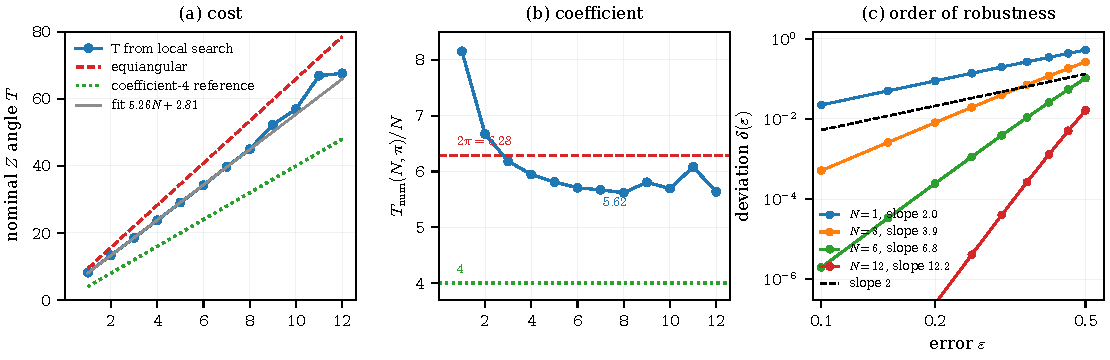
\includegraphics[width=0.93\linewidth]{fignum_num.pdf}
\caption{The same data as Table~\ref{tab:num}. (a) Cost found by the local search, against the
equiangular cost $(2N+1)\pi$ and the coefficient-$4$ line $4N$; the straight line is the fit
$T\approx5.26N+2.81$ to the branch $N\le8$, whose residuals are below $0.12$. (b) The same cost
divided by $N$, against the proved lower bound $4$ and $(2N+1)\pi/N$; the dashed line is
$2\pi\approx6.28$, which the values at $N=1,2$ exceed. (c) The deviation $\delta(\eps)$ on a
log-log grid for $N=1,3,6,12$, with its local slope; the dashed line has slope $2$, the smallest
order appearing in the figure, and each curve is drawn only while $\delta$ stays above the
round-off floor.}
\label{fig:num}
\end{figure}

\paragraph{What the numbers say.}
Write $T_{\mathrm{num}}(N,\pi)$ for the cost of the sequence found at order $N$; by construction
$T_{\min}(N,\pi)\le T_{\mathrm{num}}(N,\pi)$, and the two need not be equal. Over the range in
which the search depth is uniform, $N\le8$, those upper bounds increase by $5.2\pm0.3$ per
order,
\[
T_{\mathrm{num}}(N,\pi)\approx5.26\,N+2.81 ,
\]
with increments $5.20,5.20,5.24,5.27,5.19,5.45,5.26$ and residuals below $0.119$. Every ratio
$T/[(2N+1)\pi]$ lies between $0.839$ and $0.926$, and every ratio $T/N$ stays above the proved
coefficient $4$: it exceeds $2\pi$ at $N=1,2$ and falls below it from $N=3$ on, reaching its
smallest value $5.62$ at $N=8$. Part of the gain over the equiangular family may come from the
free angles alone---that family fixes every $\alpha_j$ at $\pi$ for algebraic
convenience, whereas~\eqref{eq:numproblem} leaves them free---but how much of it is available in
this way is a question these numbers do not answer.

\paragraph{Status of the numbers, and what they do not claim.}
The optimization is a local search with no certificate of optimality, and what
Sec.~\ref{sec:numerics} verifies is \emph{only} that each printed sequence is admissible.
Every entry of Table~\ref{tab:num} is therefore an upper bound for $T_{\min}(N,\pi)$, and
nothing more. In particular:

\begin{itemize}[leftmargin=1.4em,itemsep=0.15em,topsep=0.25em]
\item The values are \emph{not} claimed to be optimal. A cheaper sequence of the same order may
  exist, and $T_{\min}(N,\pi)$ may be strictly smaller than every number listed; these numbers give no lower bound at any finite order.
\item No asymptotic claim is made. The fit $T\approx5.26N+2.81$ describes eight upper bounds with
  residuals below $0.119$; it is not an estimate of $\cstar(\pi)$, which these numbers cannot bound
  from either side. Because the quality of the search is itself $N$-dependent---the rows $N\ge9$
  come from a different seeding and are visibly looser---the increments of Table~\ref{tab:num}
  cannot be extrapolated in $N$.
\item The segment numbers $L$ are those found by the search, not the smallest possible ones, and
  the comparison with the equiangular family is made at equal order $N$ only.
\end{itemize}

None of this section enters the proofs of Theorems~\ref{thm:elementary}, \ref{thm:jensen}
and~\ref{thm:newrung}. The one statement the data do establish is independent of optimality: the
equiangular cost $(2N+1)\pi$ is not optimal at any order considered, since every listed cost is
strictly below it, by a factor between $0.839$ and $0.926$. Closing the gap
$4\le\cstar(\pi)\le2\pi$ therefore requires either a construction in the free-$X$ model that
beats the equiangular family, or a proof that no construction attains $4$.

\section{Machine-checked verification in Lean 4}
\label{sec:formal}

Each rung of this paper corresponds to a named Lean~4 declaration of a public
development~\cite{LeanRepo}. The analysis core and the exact-criterion rung live in the
\lean{wC} tree, the Jensen rung in the \lean{wF} tree, and the weak-constant $8/\mathrm{e}$ variant in
the \lean{wM} tree (paths below are relative to \lean{lean_sharp/}). In each tree the model
-- the rotations, the evolution, \lean{Admissible}, and the cost $T=\texttt{cost}\,\theta$ --
is fixed in \lean{RobustZ/Statement.lean}, and the scalar flatness~\eqref{eq:hflat} is derived
from the matrix flatness (\lean{h_flat}) rather than assumed. Write $q=2N+2$ and
$\tauvar=T/2$.

\subsection{The machine-checked statements}

\begin{theorem}[Elementary bound, all orders; \lean{elementary_bound}, \lean{elementary_bound_pi}]
\label{thm:formal-elementary}
For every $0<\phi\le\pi$ and every order-$N$ admissible sequence,
\begin{equation}
T\ge2\,\bigl(2\,q!\,\sin^{2}(\phi/4)\bigr)^{1/q},
\qquad\text{and at }\phi=\pi:\quad T\ge2\,(q!)^{1/q}.
\label{eq:formal-elementary}
\end{equation}
This is the kernel-checked form of~\eqref{eq:thm-elementary} (Theorem~\ref{thm:elementary}).
\end{theorem}

\begin{theorem}[Jensen bound; \lean{jensen_rung_final}, \lean{jensen_rung_pi_final}]
\label{thm:formal-jensen}
For every $0<\phi\le\pi$ and every order-$N$ admissible sequence, with
$s=2\sin^2(\phi/4)$,
\begin{equation}
T\ge\frac{\pi\,q}{\mathrm{e}\,(2/s)^{1/q}},
\qquad\text{and at }\phi=\pi:\quad
T\ge\frac{\pi\,q}{\mathrm{e}\,2^{1/q}}.
\label{eq:formal-jensen}
\end{equation}
This is the kernel-checked form of~\eqref{eq:thm-jensen} (Theorem~\ref{thm:jensen}); the
ratio of the per-$N$ bound to $N$ tends to $2\pi/\mathrm{e}$ (\lean{jensen_ratio_tendsto}).
\end{theorem}

\begin{theorem}[Exact criterion; \lean{new_rung_final}]
\label{thm:formal-newrung}
Let $N\ge1$, $0<\phi\le\pi$, $1\le\tauvar<q=2N+2$. If
$\mathrm{nrCcal}(\tauvar,q)\,q^2\,\mathrm{nrE2star}(\tauvar,q)<\sin^2(\phi/4)$ with the
closed forms~\eqref{eq:besseldefs}--\eqref{eq:ccal}, then every order-$N$ admissible
sequence satisfies $2\tauvar<\mathrm{cost}\,\theta$.
This is the kernel-checked form of~\eqref{eq:thm-newrung} (Theorem~\ref{thm:newrung}).
The certified instances \lean{cert_N2}--\lean{cert_N4} and
\lean{cert_N5_tight}--\lean{cert_N12_tight} (Table~\ref{tab:certs}) and the
closed form $T\ge4(N+1)(1-\mathrm{nrU}(q))$ (\lean{nr_closed_form},
i.e.~\eqref{eq:closedform}) are proved from it with nothing else added.
\end{theorem}

\subsection{Statement-by-statement correspondence}

\begin{table}[t]\centering\footnotesize
\caption{Correspondence between the objects of this paper and the declarations that check them.
File paths are relative to \lean{lean_sharp/}; declaration names are exact.}
\label{tab:formal-correspondence}
\begin{tabular}{@{}p{0.30\linewidth}p{0.36\linewidth}p{0.30\linewidth}@{}}
\toprule
\textbf{Paper object} & \textbf{Lean declaration} & \textbf{File}\\
\midrule
\raggedcell Model, \lean{Admissible} and \lean{cost} & \raggedcell \lean{Admissible}, \lean{cost} & \raggedcell \lean{wC/RobustZ/Statement.lean} (same in \lean{wF}, \lean{wM})\\
\raggedcell Direct bound (8), Theorem~\ref{thm:direct} & \raggedcell paper-level proof (in text) & \raggedcell Sec.~\ref{sec:elementary}\\
\raggedcell Carrier flatness (20), moments (39) & \raggedcell \lean{h_flat}, \lean{h_moments} & \raggedcell \lean{wC/RobustZ/Flatness.lean}, \lean{wC/RobustZ/ExpSum.lean}\\
\raggedcell Elementary bound, Theorem~\ref{thm:elementary} & \raggedcell \lean{elementary_bound}, \lean{elementary_bound_pi} & \raggedcell \lean{wC/RobustZ/ElementaryBound.lean}\\
\raggedcell Jensen bound, Theorem~\ref{thm:jensen}, with its analytic core & \raggedcell \lean{jensen_rung_final}, \lean{jensen_rung_pi_final}, \lean{jensen_ratio_tendsto} & \raggedcell \lean{wF/RobustZ/JensenBridge.lean}, \lean{wF/RobustZ/JensenRung.lean}\\
\raggedcell Coefficient bound L1, tail sum L2 & \raggedcell \lean{fcoef_sharp}, \lean{bessel_L1}, \lean{bessel_L2} & \raggedcell \lean{wC/RobustZ/BesselTail.lean}\\
\raggedcell Realization L3, Fourier inversion & \raggedcell \lean{kap_L1_le}, \lean{realize_L1}, \lean{inversion_on_band} & \raggedcell \lean{wC/RobustZ/RealizeLemma.lean}, \lean{wC/RobustZ/InversionId.lean}\\
\raggedcell Chebyshev derivative bundle D1 & \raggedcell \lean{cb_term1_le}, \lean{cb_term2_le}, \lean{cb_hasSum0}--\lean{cb_hasSum2} & \raggedcell \lean{wC/RobustZ/ChebBundle.lean}\\
\raggedcell Exact criterion L4/L5 and closed form, Theorem~\ref{thm:newrung} & \raggedcell \lean{nr_sup_le}, \lean{nr_D1_le}, \lean{nr_D2_le}, \lean{nr_kappa_le}, \lean{nr_main_rung}, \lean{nr_closed_form} & \raggedcell \lean{wC/RobustZ/NewRung.lean}\\
\raggedcell Wrapper and finite-$N$ certificates & \raggedcell \lean{new_rung_final}, \lean{cert_N2}--\lean{cert_N4}, \lean{cert_N5_tight}--\lean{cert_N12_tight} & \raggedcell \lean{wC/RobustZ/RungFinal.lean}, \lean{wC/RobustZ/RungTight.lean}\\
\raggedcell Weak-constant $8/\mathrm{e}$ variant & \raggedcell \lean{eight_over_e_bound} & \raggedcell \lean{wM/RobustZ/EightOverE.lean}\\
\bottomrule
\end{tabular}
\end{table}

\subsection{Scope of the verification}

Machine-checked: the model and the carrier flatness; the elementary bound with its exact
constant $2$, at every order and every $0<\phi\le\pi$; the Jensen bound with its exact
constant $\pi/\mathrm{e}$ at every order and every $0<\phi\le\pi$; the exact criterion with its
closed forms, hence every entry of Table~\ref{tab:certs} and the coefficient-$4$ closed
form; and the $8/\mathrm{e}$ variant with $C=10^8$. Not machine-checked: the numerical material of
Sec.~\ref{sec:numerics}. The low-order sequences found by local search and their
re-verified costs are upper bounds computed outside Lean; they enter no proof, and no
optimality or small-$N$ statement about them is formalized. The passage from the
per-sequence bounds to $\cstar(\phi)\ge4$ in Corollary~\ref{cor:allN} is ordinary analysis
in the paper; the developments state per-sequence cost bounds and claim no formalized
infimum. The audit ran on the development sources: a source scan finds no \lean{sorry},
\lean{admit}, or \lean{axiom} in the project files, and the headline theorems depend only
on the three standard logical axioms \lean{propext}, \lean{Classical.choice} and
\lean{Quot.sound} (see the \lean{Audit*.lean} files, e.g.\
\lean{wC/RobustZ/AuditRungFinal.lean}). Statements, build logs and the raw
\texttt{\#print axioms} output are collected at \url{https://show.dytchem.cn/lean/}, and the
repository is cited as~\cite{LeanRepo}, with sources at
\url{https://github.com/Dytchem/robust-z-lower-bound-lean}.

\subsection{Code, data, and reproducibility}
\label{sec:resources}

Everything used in this paper is public: the proofs are a Lean development, the numerical sequences
and their independent re-verification are a data set with a browser front end, and the figures and
tables of Sec.~\ref{sec:numerics} are regenerated from that data by short scripts.
Table~\ref{tab:resources} collects the four entry points.

\begin{table}[t]\centering\footnotesize
\caption{Public resources for this paper. The Lean development is self-contained: a fresh clone
reproduces its statements with the three commands of its \texttt{README}. The numerical
re-verification is likewise reproducible from the last entry, which carries the sequences at the
precision used in Table~\ref{tab:num}. All addresses were accessed on 8 October 2026.}
\label{tab:resources}
\begin{tabular}{@{}p{0.22\linewidth}p{0.68\linewidth}@{}}
\toprule
\textbf{Resource} & \textbf{Content} \\
\midrule
\raggedcell \url{https://show.dytchem.cn/bloch/} &
\raggedcell Bloch-sphere animation and the full angle lists of every sequence of
Table~\ref{tab:num}; browser-side re-computation of the nominal mismatch, of the deviation
$\delta(\eps)$ and of its slope, with the equiangular family shown side by side.~\cite{DataRepo} \\
\raggedcell \url{https://show.dytchem.cn/lean/} &
\raggedcell Verification status of the formal development: the exact Lean statements of the
bounds, the source scan for \lean{sorry} and \lean{axiom}, and the raw \lean{lake build} and
\texttt{\#print axioms} output for the headline theorems.~\cite{LeanRepo} \\
\raggedcell \href{https://github.com/Dytchem/robust-z-lower-bound-lean}{GitHub repository} &
\raggedcell Lean~4 with Mathlib, pinned by \lean{lean-toolchain} and
\lean{lake-manifest.json}; \lean{VERIFICATION.md} records two from-scratch verifications on
three trees: \lean{lean_sharp/wC} carries the analysis core, the exact-criterion rung and its
certificates (52 modules); \lean{lean_sharp/wF} carries the Jensen rung and its bridge
(35 modules); \lean{lean_sharp/wM} carries the $8/\mathrm{e}$ variant (47 modules); all build
green with no \lean{sorry} or \lean{axiom} in the sources.~\cite{LeanRepo} \\
\raggedcell \href{https://show.dytchem.cn/files/code.zip}{Verification scripts and data} &
\raggedcell \lean{verify_num.py}, which rebuilds every propagator with
\lean{scipy.linalg.expm} and re-evaluates the Taylor coefficients of Sec.~\ref{sec:numerics}
at $50$ decimal digits; \lean{make_outputs.py}, which regenerates Figs.~\ref{fig:num}
and~\ref{fig:phys} and the printable angle lists of Appendix~\ref{app:sequences} from the
verified data; the data themselves (\lean{num_results.json}, \lean{solutions_largeN.json}); and
a \lean{README}.~\cite{DataRepo} \\
\bottomrule
\end{tabular}
\end{table}

Each tree builds green from its pinned toolchain and manifest alone.
The angle lists of Appendix~\ref{app:sequences} are stored in the convention in which they were
verified, rounded to $12$ decimals of $\pi$; the rounding is checked, not assumed: feeding those
rounded lists back into~\eqref{eq:rotations}--\eqref{eq:robustness} again gives a nominal
mismatch below $9\times10^{-10}$ and a flatness residual below $1.5\times10^{-10}$, which are the
two accuracy statements of Table~\ref{tab:num}.


\section{Discussion}
\label{sec:discussion}

The bounds are lower bounds on a resource, not a pulse-design prescription. Free and
exact $X$ rotations can rearrange how the systematic $Z$ error accumulates, but when the
common $Z$ scale is turned down to $\lambda=0$ every costly evolution disappears, and the
carrier must connect two separated endpoints while being extremely flat at $\lambda=1$.

\subsection{What the ladder rules out and the orders that matter}

At every order the cost is bounded below by the
elementary bound, hence by $4(N+1)/\mathrm{e}$: no arrangement of free rotations, however many,
makes high-order robustification sublinear. The exact-criterion rung gives $\cstar(\pi)\ge4$; the equiangular family of~\cite{Low2014} gives $\cstar(\pi)\le2\pi$, so
\begin{equation}
4\;\le\;\cstar(\pi)\;\le\;2\pi ,
\label{eq:window}
\end{equation}
an interval of width $2\pi-4\approx2.28$, whose endpoints differ by the factor $\pi/2$; the numerical costs of
Sec.~\ref{sec:numerics} follow $T\approx5.26N+2.81$ over $N\le8$, within a factor
$2.0$ of the floor at $N=1$ and $1.4$ at $N=8$, so what remains to be found is a bounded correction rather than a new
regime. Moreover, the model already grants the designer everything a fast-control layer could
offer---exact, instantaneous and free $X$ rotations in unlimited number and at arbitrary
positions, with the target reached exactly at the nominal error---and the bound is still linear:
here, a rich enough fast-control layer does not make the uncertain evolution asymptotically
efficient.

\paragraph{Why the idealization makes the bounds conservative.} The model is thin by design and every assumption favors the designer: one common multiplicative error, no time dependence, no decoherence, no leakage, instantaneous and perfect transverse control. Any model closer to a laboratory adds constraints, and adding constraints can only raise the least cost of an order-$N$ robust sequence.

\paragraph{Finite order, incoherent errors, and the orders that matter.} A device does
not get to choose $N$ freely: a longer sequence also spends more time in the presence of
decay, the tension that shapes time-optimal gate design on Rydberg platforms~\cite{Jandura2022}. Writing $\omega$ for the rate at which the uncertain $Z$-phase
accumulates and $\gamma$ for the decay rate, an order-$N$ sequence of cost $T$ pays an
incoherent infidelity of order $\gamma T/\omega$ while its coherent error falls like
$\eps^{N+1}$, and the two balance at
\begin{equation}
N^\ast\;\approx\;\frac{\ln(\omega/\gamma)}{2\ln(1/\eps)},
\label{eq:nstar}
\end{equation}
so the useful order grows only logarithmically as coherence improves. At the parameters of Fig.~\ref{fig:phys} the estimate gives $N^\ast\approx3.0$, up to the order-one prefactor of the coherent term; the tabulated sequences place the minimum at $N^\ast=2$.

This is where the
finite-order form of the bounds matters: the relevant orders are small, and there the
operative terms of~\eqref{eq:allN} are the elementary and Jensen rungs, which supply the cost side of
the balance at every order and without a threshold. The tradeoff
cannot be evaded by inventing better pulses, only by improving $\gamma$, $\eps$, or the
resource model itself. Figure~\ref{fig:phys} evaluates the balance at parameters
representative of current neutral-atom arrays: the optimum is at $N^\ast=2$, and improving
$\gamma/\omega$ by three orders of magnitude moves it only to $4$.

\begin{figure}[t]\centering
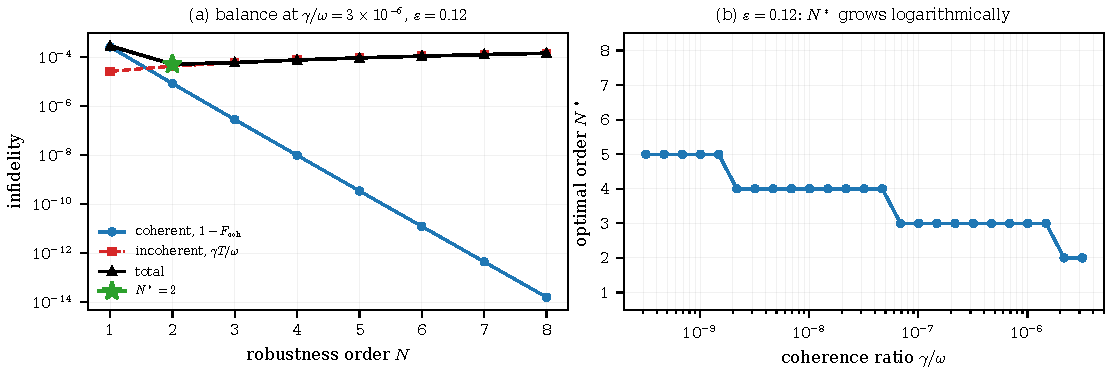
\includegraphics[width=0.93\linewidth]{figphys.pdf}
\caption{The coherent-versus-incoherent balance at parameters representative of current
neutral-atom arrays: interaction strengths $V/2\pi$ of a few hundred MHz at
few-micrometre separations~\cite{Evered2023,Mohan2023} and Rydberg lifetimes of order
$10^2\,\mu$s~\cite{Beterov2009}, which for $V/2\pi=500$~MHz and $\gamma/2\pi\approx1.6$~kHz
give a coherence ratio $\gamma/\omega\approx3\times10^{-6}$, together with a systematic
variation $\eps=0.12$. (a) Coherent
infidelity $\sin^2(\delta(\eps)/2)$ of the sequences of Table~\ref{tab:num}, the incoherent
infidelity $\gamma T/\omega$ they accumulate, and the sum; the minimum is at $N^\ast=2$. (b) The
same balance over four decades of the coherence ratio; the optimum moves only to $N^\ast=4$
after three decades and to $N^\ast=5$ after four. The
sequences plotted are those of Table~\ref{tab:num} with $N\le8$, and the coherent term is
measured for them, so it is an upper bound on what a better construction of the same order could
reach.}
\label{fig:phys}
\end{figure}

\subsection{Negatives: what cannot improve the ladder}

\paragraph{No third algebraic doubling.} The replacement method uses only two pieces of
information: the band $|\mu_m|\le\tauvar$ and the flatness $h^{(k)}(1)=0$, $k<q$, with
$q=2N+2$. The class
of admissible replacements is already maximal: if a continuous function $Q$ satisfies
$\sum_m\gamma_mQ(\mu_m)\mathrm{e}^{\mathrm{i}\mu_m}=0$ for every admissible sequence, then
$Q|_{[-\tauvar,\tauvar]}$ is a polynomial of degree $<q$ (Hahn--Banach: the annihilator of
the twisted moment measures in $C([-\tauvar,\tauvar])$ is the uniform closure of
$\Pi_{q-1}$, which equals $\Pi_{q-1}$ since a finite-dimensional subspace is closed). In
particular, no determinant, character identity, or higher trace power can add a new
functional. Moreover, products preserve the flatness-to-band ratio: if $h_1,h_2$ have
bands $\tauvar_1,\tauvar_2$ and flatness orders $q_1,q_2$ at $1$, then $h_1h_2$ has band
$\tauvar_1+\tauvar_2$ and flatness order $q_1+q_2$, so the threshold $\tauvar<q$ -- the
source of the coefficient~$4$ -- is unchanged by any power trick. The one explicit
square-root variant is strictly worse because it halves the order: writing
$V_\lambda=U_1^\dagger U_\lambda=a+\mathrm{i}\mathbf{b}\cdot\bm{\sigma}$ gives
$h=|\mathbf{b}|^2/(1+a)$, where each component $b_j$ has band $\tauvar$ but flatness only
$N+1$, so that route needs $\tauvar\lesssim N+1$, i.e.\ asymptotic coefficient~$2$. There
is no third doubling of the coefficient, only a reparametrisation.

\paragraph{The minimax polynomial is marginal.} Let $E_{q-1}(\tauvar)$ be the best uniform
approximation error of $\mathrm{e}^{-\mathrm{i}\mu}$ on $[-\tauvar,\tauvar]$ by degree-$<q$ polynomials, and
let $\varepsilon^{\mathrm{tr}}$ be the Chebyshev-truncation error used by the rung. The
$L^2$ argument with the Chebyshev probability weight gives
$\sqrt2\,|c_q|\le E_{q-1}(\tauvar)\le\varepsilon^{\mathrm{tr}}\le2\sum_{k\ge q}|c_k|$,
so replacing the truncation by the optimal polynomial improves the error by at most a
constant factor. Since the rung criterion is a condition on the error at the log level, a
constant factor shifts the exponent by an additive constant only, and the asymptotic
coefficient stays~$4$.
\begin{remark}[Numeric illustration, not a theorem]
Relaxing the error threshold by a factor $F=2$ changes the computed $N=12$ value by about
$+3.4\%$; larger relaxations add a few further percent. These are computed illustrations
only: the minimax direction is a refinement, never a new rung.
\end{remark}

\paragraph{The free $X$-angle gives nothing at $\phi=\pi$.} The exact endpoint identity
is $h(0)=1-\cos(\phi/2)\cos(A/2)$ with $A=\sum_j\alpha_j$ free. At $\phi=\pi$ one has
$\cos(\phi/2)=0$, so $h(0)=1$ for every $A$: no parity, topological, or other constraint
on $A$ can improve the endpoint bound in the worst case, which is the case the theorem is
about. At $\phi<\pi$, $\min_Ah(0)=1-\cos(\phi/2)=2\sin^2(\phi/4)$, attained at
$A\equiv\pi$, which is exactly the bound used here. The genuinely larger endpoint
constant $|\mathbf{b}(0)|\ge\sin(\phi/2)$ belongs to the halved-order $\mathbf{b}$-vector
route above, which is strictly worse.

\subsection{Ceiling: the dichotomy at $4$ and the open gap}

Can any argument using only the band data (band $\tauvar$, flatness order $q=2N+2$ at
$\lambda=1$, $\|h\|_\infty\le2$, endpoint $h(0)\ge2\sin^2(\phi/4)$) certify
$\liminf T/N>4$? The answer is equivalent to one exact obstruction. Call $\mathrm{UP}(q)$
the statement that there exist bandwidth $q$ and a compactly supported density whose
Fourier transform is $2^{-q}$-small at $O(1)$ distances from its peak while carrying
endpoint $>1$ at sup $\le2$. Two implications fix the status of the ceiling. If
$\mathrm{UP}(q)$ holds for every $q$, then no band-data argument certifies a coefficient
larger than $4$: a witness at bandwidth $q=2N+2$ satisfies every hypothesis used at order
$N$ while realizing $T=2q\approx4N$, so no argument built from those hypotheses can exclude
it. Conversely, if $\mathrm{UP}(q)$ fails for some $q$, then the band data at that order
already exclude bandwidth $q$, and the ceiling is not forced by the data there. Whether the
ceiling at $4$ holds is thus decided exactly when this uncertainty principle is decided for
all large $q$, and this paper takes no position on it.

The ceiling at $4$ is \emph{open}. What is proved is the diagnosis on both sides. Every
natural candidate witness family fails $\mathrm{UP}(q)$ by the same quantitative
mechanism -- edge diffraction amplified by $|\cdot|^q$: sine powers give the $2\pi$
witness below but fail at $4$; polynomial bumps, Gaussians with any cutoff width, and
lattice profiles all fail with the endpoint-to-supremum ratio decaying exponentially in
$q$. Nor is $\mathrm{UP}(q)$ cheap to refute: no elementary argument eliminates it. What is
known unconditionally is threefold: the rung with coefficient $4$
(Theorem~\ref{thm:newrung}); a universal band-data cap at $2\pi$, proved by a Rolle
alternation argument ($\cos$ takes alternating values $(-1)^k$ at $k\pi$, forcing the real
part of any approximating polynomial to be constant once $\tauvar\ge\pi q/2$, so the error
is at least $1$), with the extremal witness $g(x)=2\sin^q(\pi x/2)$ of type $\pi q/2$
attaining the endpoint $2$; and the necessity that any admissible kernel has $L^1$ norm at
least the best-approximation error. Thus $[4,2\pi]$ is the exact open gap for band-data
methods, sharp at the upper end by the equiangular family, and this paper takes no position
on whether the ceiling at $4$ holds or fails.

\paragraph{Thresholds and numerics.} The closed-form threshold of~\eqref{eq:closedform} is
a sufficient condition assembled from explicit majorants -- a contour-shift coefficient
bound, a geometric tail sum, and kernel bookkeeping. The constant $6$ and the threshold
$500+\lceil\exp((11+|\log s_0|)/1.2)\rceil$ are conservative bookkeeping rather than
features of the control problem. The criterion~\eqref{eq:thm-newrung} being unverified
below a certified bandwidth is therefore not evidence that the coefficient is smaller
there; those orders are covered by the elementary and Jensen rungs.


\subsection{Conclusions}

The cost of cancelling a common systematic error to order $N$ in the free-$X$ model is
linear in $N$, and the four rungs of this paper pin down how much of the coefficient is
accessible to successively stronger arguments: $2/\e$ and $4/\e$ from one Taylor step,
$2\pi/\e$ once the carrier is treated as an entire function of exponential type, and a
coefficient approaching $4$ once its whole band is used. What is proved is therefore both a
statement about the resource and a statement about the method: the ladder closes at $4$ for
every argument that uses only the bandwidth, the flatness order, the supremum bound and the
endpoint separation, the gap $[4,2\pi]$ is what remains in this model, and at the small orders
that a device with realistic coherence actually uses the elementary and Jensen rungs already
supply the operative bound. The numerical sequences show that the equiangular family is not
optimal at any order considered, so the upper end is not rigid either. Extending any of these
statements---to non-common errors, to a full account of decoherence, or to a proof that the
ceiling at $4$ is attained or violated---would move the window, not the ladder.


\begin{acknowledgments}
The author thanks the Lean~4 and Mathlib communities, whose libraries and tooling made the
formal verification possible.
\end{acknowledgments}

\section*{Data availability}
The Lean~4 formalization~\cite{LeanRepo} and the numerical data set with its verification
scripts~\cite{DataRepo} are openly available; both were accessed on 8 October 2026. The formal
development builds from a fresh clone with its pinned toolchain and manifest, and the data set
contains the angle lists behind Table~\ref{tab:num}, the propagator re-verification, and the
scripts that regenerate Figs.~\ref{fig:num} and~\ref{fig:phys} and the tables of
Sec.~\ref{sec:numerics}.

\appendix

\section{Exact-criterion rung: closed forms and kernel estimate}
\label{app:technical}

This appendix states verbatim, in Lean's notation, the technical lemmas behind
Theorem~\ref{thm:newrung}: the contour-shift coefficient bound, the collar bookkeeping, and
the smoothing-kernel estimate. (The fourth technical ingredient, the flatness doubling of
Proposition~\ref{prop:flatness}, is proved in Sec.~\ref{sec:carrier}.) Nothing here adds a
claim: every constant below is the one checked by Lean.

\subsection{The closed-form quantities}

For $\tauvar>0$ and $k>\tauvar$ put
\begin{equation}
\alpha(\tauvar,k):=\operatorname{arcosh}(k/\tauvar),
\qquad
f(\tauvar,k):=k\,\alpha(\tauvar,k)-\sqrt{k^2-\tauvar^2},
\label{eq:besseldefs}
\end{equation}
(Lean \lean{besselAlpha}, \lean{besselF}). The tail majorant and its closed-form sum are
\begin{equation}
B(k):=\sqrt{\frac{\pi}{8}}\,
\frac{\mathrm{e}^{-f(\tauvar,k)}}{(k^2-\tauvar^2)^{1/4}},
\qquad
E_2^\ast(\tauvar,q):=
\frac{2\sqrt{\pi/8}\;\mathrm{e}^{-f(\tauvar,q)}}
{\sqrt{\sqrt{q^2-\tauvar^2}}\;\bigl(1-\mathrm{e}^{-\alpha(\tauvar,q)}\bigr)},
\label{eq:e2star}
\end{equation}
(Lean \lean{majorB}, \lean{nrE2star}), with $E_2(\tauvar,q):=2\sum_{m\ge0}B(q+m)\le
E_2^\ast(\tauvar,q)$ (Lean \lean{nrE2_le_E2star}, from \lean{bessel_L2}). The weighted
tail factors are, with $r=\mathrm{e}^{-\alpha(\tauvar,q)}$,
\begin{equation}
\eta_1(r):=\frac{1+r}{(1-r)^3},
\qquad
\eta_2(r):=\frac{1+11r+11r^2+r^3}{(1-r)^5},
\label{eq:eta12}
\end{equation}
(Lean \lean{nrEta1}, \lean{nrEta2}), and the collar width is $B_c:=\tauvar/q^2$ (Lean
\lean{nrB}). Assembling the realization bound of the next subsection at this width gives
the calibration factor
\begin{equation}
\mathrm{nrCcal}(\tauvar,q)
:=\frac{2}{\pi}\,\frac{1}{q}\,
\sqrt{\,2\Bigl(1+\frac{B_c}{\tauvar}\Bigr)
\Bigl(1+\frac{4}{27}\eta_1\Bigr)
\Bigl(32\,\eta_2\,q^2+44+2\Bigl(12+\frac{16}{27}\Bigr)\eta_1\Bigr)\,}\,.
\label{eq:ccal}
\end{equation}
where the square root covers the whole product (Lean \lean{nrCcal}; here
$\eta_i=\eta_i(\mathrm{e}^{-\alpha(\tauvar,q)})$). The coefficient bound behind~\eqref{eq:e2star}
is \lean{fcoef_sharp} (headline \lean{bessel_L1}); the tail sum is \lean{bessel_L2}.

\subsection{Realization and the kernel bound}

Let $\Psi=\mathrm{e}^{-\mathrm{i}\cdot}-P$ with $P$ the degree-$(q-1)$ Chebyshev truncation, and let
$\chi$ be the explicit $C^2$ cutoff with $\chi=1$ on the band, supported in the collar,
and $\|\chi'\|\le K/B_c$, $\|\chi''\|\le K/B_c^2$ with $K=4$. The development builds a
kernel $\kappa\in L^1(\R)$ whose Fourier transform agrees with $\Psi$ on the band
(Lean \lean{inversion_on_band}) and controls its $L^1$ norm by the split-point
optimization (Lean \lean{kap_L1_le}, headline \lean{realize_L1}):
\begin{equation}
\displaystyle
\int_\R\|\kappa(t)\|\,\mathrm{d}t
\;\le\;
\mathrm{nrCcal}(\tauvar,q)\,q^2\,\mathrm{nrE2}(\tauvar,q).
\label{eq:kernelbound}
\end{equation}
The inputs are the band error $\|\Psi\|\le\mathrm{nrE2}$ (Lean \lean{nr_sup_le}) and the
derivative bounds through the Chebyshev tail (Lean \lean{nr_D1_le}, \lean{nr_D2_le},
assembled in \lean{nr_kappa_le}). With $\mathrm{nrE2}\le\mathrm{nrE2star}$ this is the
quantitative heart of the proof: all dependence on $\tauvar$ has disappeared except for
the hypothesis $\tauvar<q$.

The scope distinctions are recorded in Sec.~\ref{sec:formal}: the elementary and Jensen
rungs and the exact criterion are machine-checked end to end, while the passage from the
per-sequence bounds to $\cstar(\phi)\ge4$ in Corollary~\ref{cor:allN} is ordinary analysis
in the paper and no formalized infimum is claimed.

\section{Numerical solutions}
\label{app:sequences}

The angle lists behind Table~\ref{tab:num} are distributed with the data set of
Ref.~\cite{DataRepo}, in the convention in which they were verified. For every order $N\le12$ at
$\phi=\pi$ the data set gives the $L$ costly angles $\theta_j$ and the $L$ free angles
$\alpha_j$ in units of $\pi$, both in the \emph{time order} of the sequence: $\alpha_j$ is the
free rotation that follows the costly segment $\theta_j$, and the first entries are the ones
applied first. The product that was verified is therefore
\[
U_\lambda=X(\alpha_L)Z(\lambda\theta_L)\,X(\alpha_{L-1})Z(\lambda\theta_{L-1})\cdots
X(\alpha_1)Z(\lambda\theta_1),
\]
which is~\eqref{eq:sequence} with the indices relabeled, $j\mapsto L+1-j$. Two conventions turn the raw
optimizer output into these lists, and both are exact rather than cosmetic: surplus free rotations,
where the search produced $L+1$ of them, are merged with $X(a)X(b)=X(a+b)$, and every $\alpha_j$ is
reduced to its representative in $[0,2\pi)$, which uses $X(\alpha+2\pi)=-X(\alpha)$ and therefore
changes the propagator only by the global sign that the convention $U_1=Z(\pi)$ of~\eqref{eq:target} restores. After those two steps each row has $L$ angles of each kind, as the
sequence of the paper requires.

Each list was re-verified from scratch in exactly this form, as described in
Sec.~\ref{sec:numerics}: the nominal mismatch $\lVert U_1\mp Z(\pi)\rVert$ is below
$9\times10^{-10}$ and the flatness residual $\rho_N$ of~\eqref{eq:Ukbound} is below
$1.5\times10^{-10}$, so the lists carry the accuracy claimed in Table~\ref{tab:num}, and the
deviations from the target follow $\eps^{N+1}$ accordingly. The same lists, with the Bloch-sphere
trajectory of every sequence and a browser-side re-computation of these numbers, are the first
resource of Table~\ref{tab:resources}. The script that regenerates this appendix in printable
form from the verified data is part of the same data set.


\bibliography{refs}

\end{document}
